\documentclass{article}%<<<
\usepackage[linktocpage=true]{hyperref}
\usepackage{graphicx}
\usepackage[utf8]{inputenc}
\usepackage{fancyvrb}
\usepackage{verbdef}
\usepackage[usenames,dvipsnames]{xcolor}
\fvset{frame=single,framesep=1mm,fontfamily=courier,fontsize=\scriptsize,numbers=left,framerule=.3mm,numbersep=1mm,commandchars=\\\{\}}
\verbdef{\mytilde}{\~}
%>>>
%Title <<<
\author{Loïc Simon}
\title{BSI TP1: Surfaces paramétriques et élimination des parties cachées}
\date{\today}

\begin{document}
\maketitle
%>>>

% Objectif <<<
L'objectif de ce TP est d'appréhender les bases de l'API d'OpenGL moderne au
travers d'une sur-couche orientée objet, et qui servira de cadre pour ce TP et
les suivants. Cette sur-couche repose, sur
la librairie GLFW pour créer un contexte OpenGL Core Profile et gérer les
interactions utilisateur.               
%>>>


\section{Instructions}%<<<
% Récupération du code et premiers tests<<<
\subsection{Récupération du code et premiers tests}
Pour ce tp, comme les suivants vous devez continuer à travailler sur le
répertoire git commun a tous les TPs. 
Pour rappel, pour compiler le projet en ligne de commande, vous devez exécuter
les commandes suivantes:
\begin{Verbatim}
  cd ${HOME}/Bureau/TPSI \textcolor{OliveGreen}{# adapter en fonction de votre configuration}
  cd GLLabs
  cd build
  make
\end{Verbatim}

Une fois la compilation terminée, vous disposez d'un exécutable que vous pouvez tester:
\begin{Verbatim}
  ./Minimal/minimal
\end{Verbatim}

Dans ce TP vous travaillerez uniquement sur le  fichier \verb|Minimal/minimal.cpp|.
Dans son état original, l'exécutable créé, affiche une scène composée d'un cube
multicolore. 

{\bf Attention!} N'oubliez pas de commiter régulièrement. Pour ce faire, vous
pouvez utiliser la commande:
\begin{Verbatim}
  git commit -am "A nice log message" \textcolor{OliveGreen}{# Adapter le message en conséquence.}
\end{Verbatim}
%>>>

%Structure du répertoire<<<
\subsection{Structure du répertoire}


Pour rappel, le répertoire est constitué de plusieurs dossiers ayant chacun leur utilité:
\begin{itemize}
\item \verb|resources| est destiné a stocker les ressources de type GLSL,
textures, maillage.
\item \verb|include| contient un unique header \verb|lightGlAPI.hpp| qui implémente l'API de la
sur-couche d'OpenGL utilisée dans les TP.
\item \verb|utils| contient des routines de plus bas niveau, utilisées dans l'API
précédente. Ces fonctionnalités proviennent pour la plupart du tutoriel:
\url{http://www.opengl-tutorial.org/}. Ces routines ne seront normalement pas
utilisées directement.
\item \verb|Minimal| contient le code nécessaire pour ce premier TP. D'autres
répertoire du même type seront ajoutés pour les autres TPs.
\end{itemize}
%>>>

% Système d'exercices<<<
\subsection{Système d'exercices}
D'autre part, dans le code, des sections sont réservées pour les réponses aux exercices. Elles sont du type:
\begin{Verbatim}
    if(controls.exercice==i)
    {
        /*!todo Instructions pour l'exercice i*/
    }
\end{Verbatim}
Une telle section doit être remplie pour l'exercice \verb|i| en suivant les
instructions en commentaire. Certaines sections sont identiques pour plusieurs exercices, et certains exercices peuvent être concernés par plusieurs sections.
\emph{Respectez bien cette structure !}

Au départ le code est incomplet pour tous les exercices à part l'exercice 0 (qui
correspond à la scène de base). Lorsque vous aurez répondu, vous pourrez
naviguer entre les différents exercices en appuyant sur la touche 'e' pour
passer à l'exercice suivant, la touche 'E' pour le précédent, ou utiliser le
pavé numérique pour passer directement à un exercice donné. 

Vous pouvez aussi obtenir une aide sur les différent raccourci clavier en tapant
'h'. L'aide s'affichera sur le terminal.
%>>>
%>>>


\section{Exercices}%<<<
\subsection{Exercice 0: Compréhension}%<<<

Prenez le temps d'analyser le code dont vous disposez déjà, de le comprendre et
de poser des questions sur les parties qui vous semblent obscures.

\begin{itemize}
  \item[Q1.] Expliquez les étapes principales pour envoyer au GPU la description
  d'un maillage. 
  \item[Q2.] Comment est spécifié le lien entre les variables du shaders ("in")
  et les attributs correspondant du VAO? Donnez les appels de routines OpenGL
  qui concrétisent ce lien.
\end{itemize}
%>>>

\subsection{Exercice 1: Activation du back-face culling}%<<<
\begin{itemize}
  \item[Q3.] Le rendu original est erroné. Expliquez à l'aide d'un schéma la
  raison de ce problème.
\end{itemize}
Activez le "back-face culling" pour éliminer ce problème.
%>>>

\subsection{Exercice 2: Création d'un tore}%<<<
En vous inspirant des fonctions équivalentes pour le cube, remplissez le corps des
fonctions utiles à la définition et au dessin du tore. 

Pour créer le maillage du tore vous utiliserez la définition du tore en tant que
surface paramétrée.
Dans un premier temps, le tore sera coloré entièrement en rouge, puis en dégradé
linéaire allant du rouge au bleu (cf. Figure \ref{fig:torus}).

\begin{figure}
  \begin{center}
    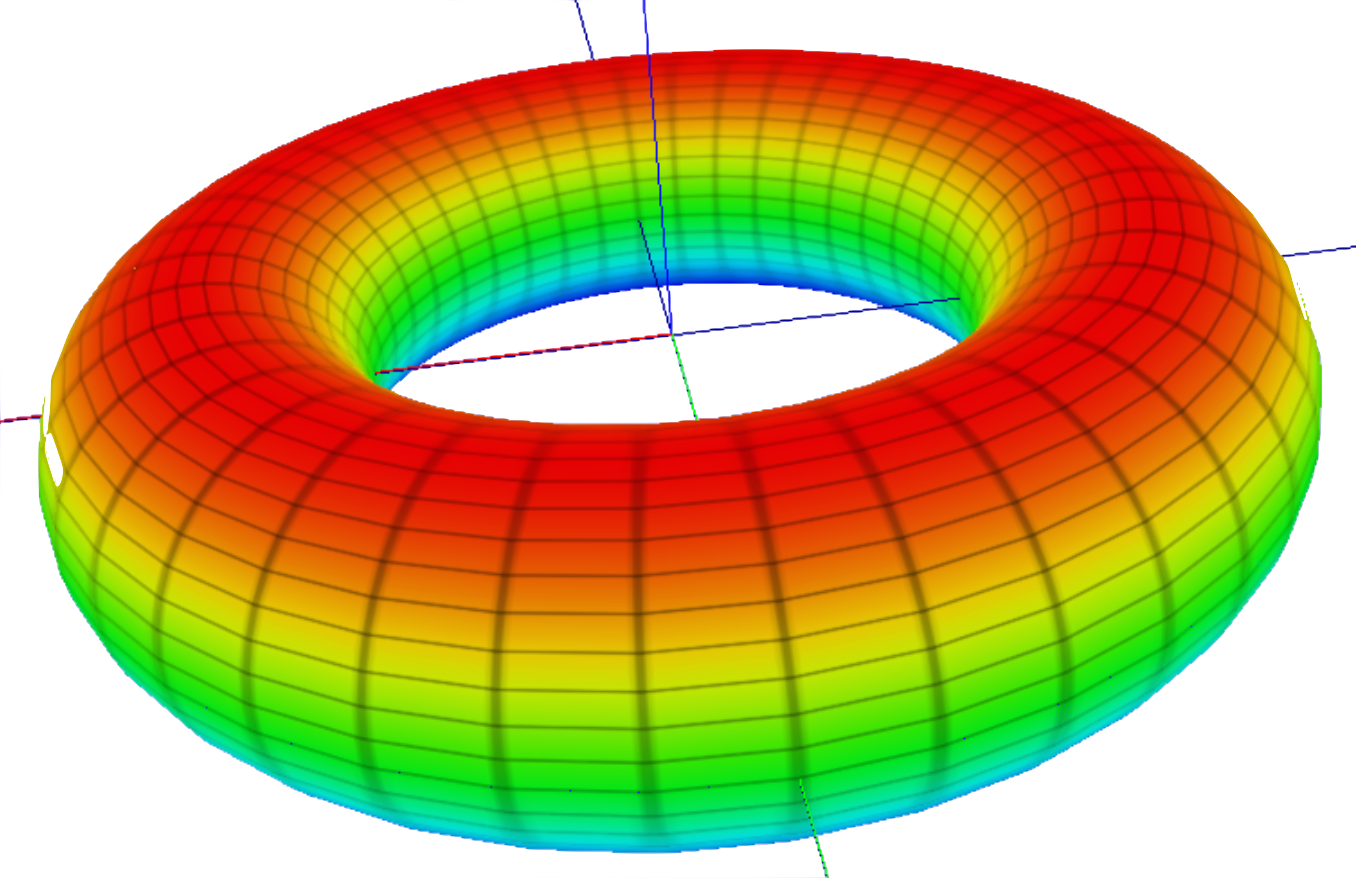
\includegraphics[width=0.7\textwidth]{torus}
  \end{center}
  \caption{Le tore en dégradé de couleur.}
  \label{fig:torus}
\end{figure}

Vous vous arrangerez par ailleurs pour
que le centre tore soit placé à une distance 1 du centre du cube.

\begin{itemize}
  \item[Q4.] Expliquez à l'aide d'un schéma la façon dont le tore est
  paramétré. Vous fournirez la formule de la paramétrisation, et l'expliquerez
  via le schéma.
  \item[Q5.] Expliquez comment vous avez obtenu la normale en un point de la
  surface du tore. Vous utiliserez une formule analytique basée sur la
  paramétrisation du tore.
  \item[Q6.] Expliquez comment vous avez entrepris le placement du tore.
  Attention, il est déconseillé de réaliser ce placement en modifiant les
  coordonnées des vertices, pourquoi?
\end{itemize}
%>>>

\subsection{Exercice 3: z-buffer}%<<<

Normalement à ce point du TP les dessins du cube et du tore doivent se
mélanger de façon incohérente. Activez le z-buffer pour éliminer ces incohérences.

\begin{itemize}
  \item[Q7.] Expliquez le pourquoi des incohérences mentionnées. Illustrez de
  façon graphique.
  \item[Q8.] Expliquez à quoi sert le z-buffer. Vous pourrez vous appuyer sur une
  description pseudo-code de l'algorithme.
\end{itemize}
%>>>

\subsection{Exercice 4: Application indépendante}%<<<

Intégrez les fonctionnalités de ce TP (cube, tore, back-face culling, z-buffer)
dans le code indépendant \verb|fromScratch/myOwnOpenGLProg.cpp|.
Par contre, vous n'utiliserez pas la
sur-couche du fichier \verb|lightGlAPI.h|.

%>>>
%>>>


\section{Compte-rendu du TP}%<<<

Tous les TPs sont a effectuer en binôme. Seul le code devra être rendu. Pour
rappel, le rendu du code sera fait grâce à votre répertoire git public qui doit
être opérationnel via le chemin suivant:
\begin{Verbatim}
  ${HOME}/public_html/gits/GLLabs.git
\end{Verbatim}

Votre chargé de TP pourra alors le récupérer via la commande:
\begin{Verbatim}
  git clone http://www.ecole.ensicaen.fr/~YOURLOGIN/gits/GLLabs.git 
\end{Verbatim}



Aucun rapport n'est obligatoire. Toutefois je vous conseille de savoir répondre
aux questions posées dans les énoncés, car elles récapitulent les points clés de ces
TP. 

%Pour le rapport, vous le rendrez sous forme d'un fichier pdf (créé avec LaTeX ou tout autre moyen qui vous convient). Je vous recommande fortement d'agrémenter votre rapport avec vos captures d'écran (images et/ou vidéos). Dans ce rapport devra figurer, les réponses aux questions formulées dans cet énoncé, ainsi que toute remarque concernant votre production et pourquoi pas votre avis sur le TP ou bien sur certains exercices.

%Vous pourrez soit rendre le fichier pdf isolé, soit dans une archive tar
%contenant des pièces annexes (vidéos, ...). Dans tous les cas, le nom du fichier
%devra être de la forme \Verb|\textcolor{red}{votrenom}_tp1_rapport.ext| où \verb|ext| $\in$
%\verb|{pdf,tar}|. Si vous optez pour une archive vous pourrez utiliser
%l'instruction:

%\begin{Verbatim}
  %tar -cf \textcolor{red}{votrenom}_tp1_rapport.tar tp1/ --exclude=".*" --exclude="*\mytilde"
%\end{Verbatim}
%ou \verb|tp1| est a remplacer par le répertoire contenant vos documents.
\begin{center}
  {\huge \it  Bon courage!}
\end{center}
%>>>

\end{document}

% vim: spelllang=fr foldmethod=marker fileencoding=utf-8:
